\subsection{Digital Twin for Remote Monitoring and Control}
\label{sec:digital_twin}

\begin{figure*}[t]
  \begin{center}
    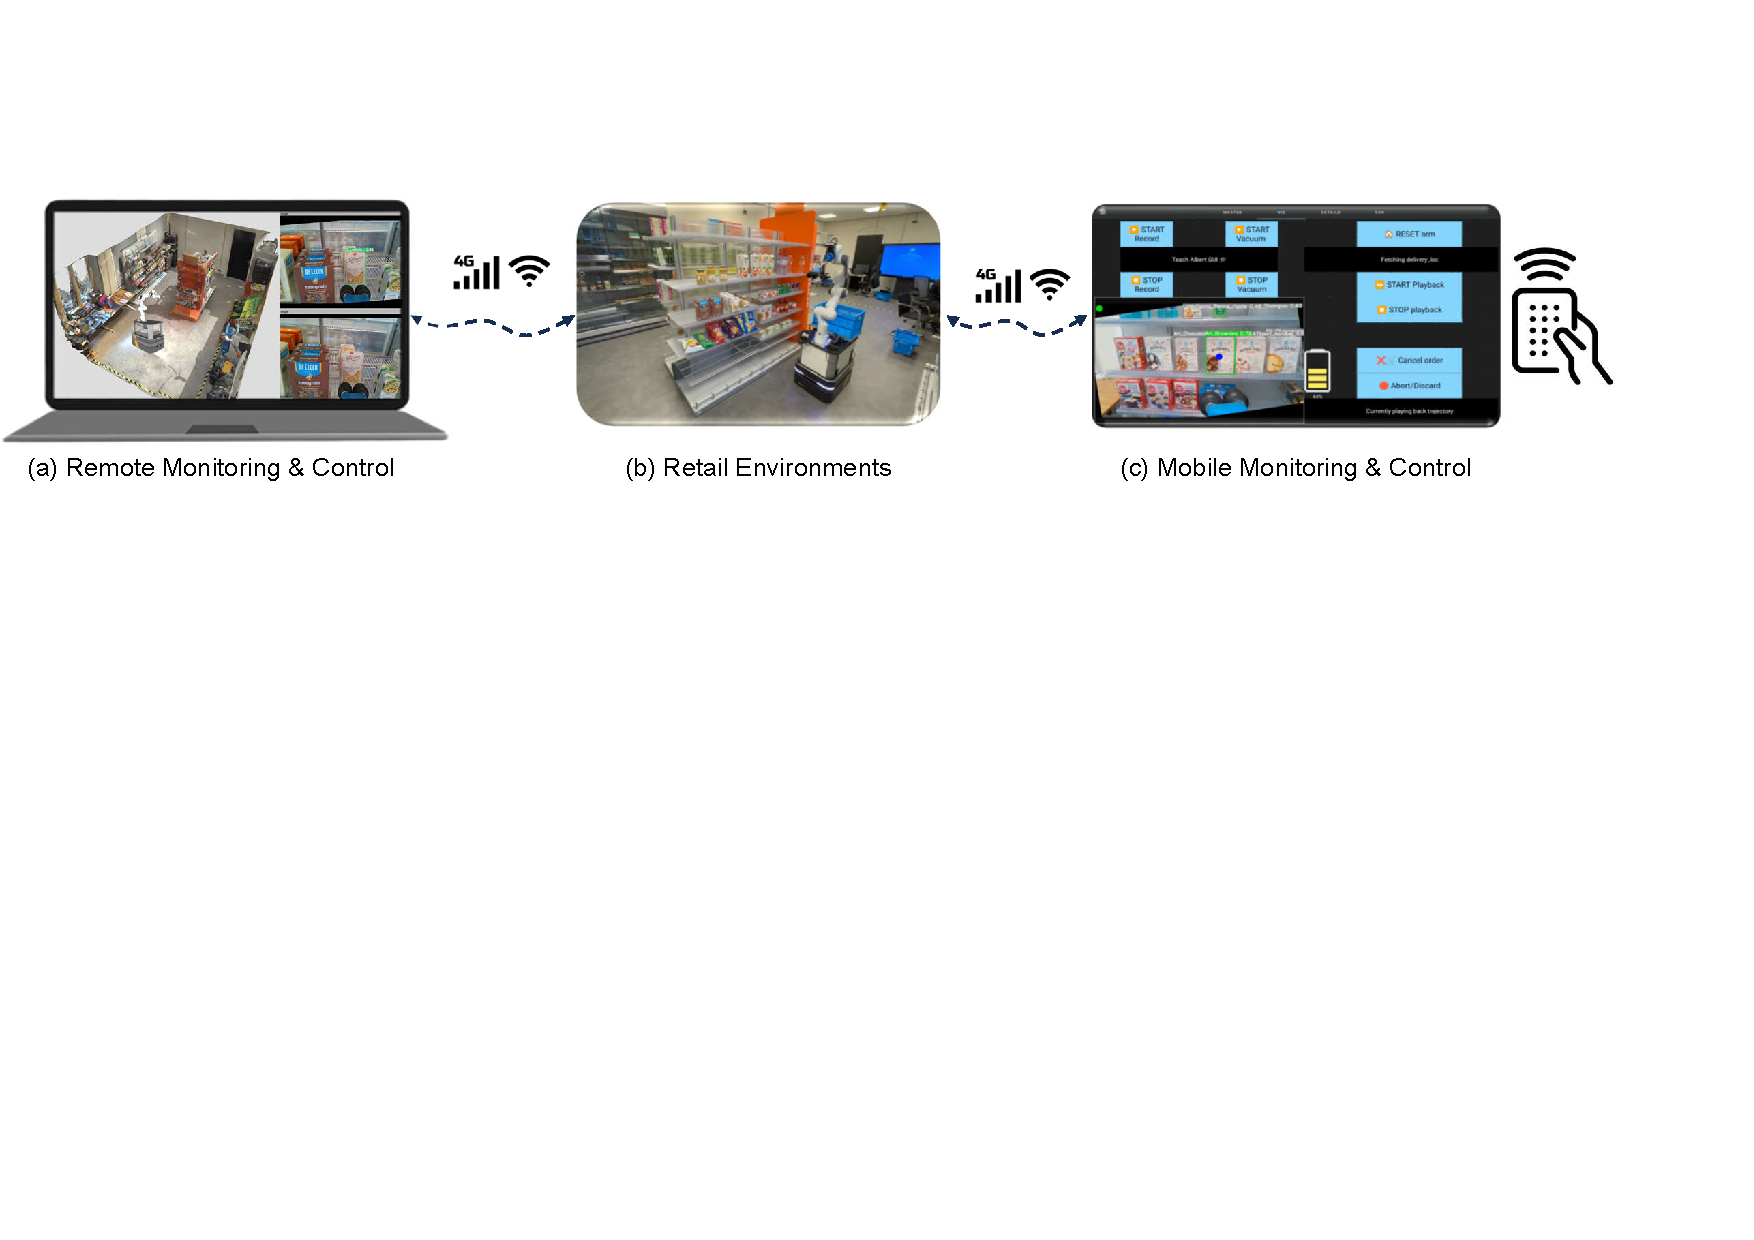
\includegraphics[width=0.85\linewidth]{remote_v5.pdf}
  \end{center}
  \caption{Overview of the remote monitoring and control
  system. a) Laptop-based remote interface for monitoring
  and control system; b) Visualization of the robot within
  the actual retail environment; c) Tablet interface for
  on-the-go monitoring and task programming.}
  \label{fig:remote_overview}
\end{figure*}

Herein, we introduce a digital twin mechanism to support
remote monitoring and control of a mobile manipulator in a
retail setting, as shown in \cref{fig:remote_overview}. By
scanning the environment in three dimensions, we construct a
virtual model that accurately represents the workspace. The
robot, when operational in a supermarket, is connected to
this digital twin through Wi-Fi or 4G, enabling operators to
monitor its status and issue commands remotely. The addition of a tablet interface allows for
flexible monitoring and control by on-site staff, who can
easily adjust the robot's course or teach it new tasks as
needed.



